
\newcommand{\D}{6} % number of dimensions (config option)
\newcommand{\U}{5} % number of scale units (config option)

\newdimen\R % maximal diagram radius (config option)
\R=3.5cm 
\newdimen\L % radius to put dimension labels (config option)
\L=4cm

\newcommand{\A}{360/\D} % calculated angle between dimension axes  

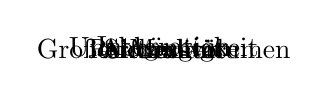
\begin{tikzpicture}[scale=1]
\def\firstcircle{\draw  [color=gray,line width=1.5pt,opacity=0.5, pattern=north west lines,pattern color=gray] (D2-3) -- (D3-4) -- (D4-4) -- (D3-3) -- (D2-3)}
\def\secondcircle{(45:2cm) circle (1.5cm)}

  \path (0:0cm) coordinate (O); % define coordinate for origin

  % draw the spiderweb
  \foreach \X in {1,...,\D}{
    \draw (\X*\A:0) -- (\X*\A:\R);
  }

  \foreach \Y in {0,...,\U}{
    \foreach \X in {1,...,\D}{
      \path (\X*\A:\Y*\R/\U) coordinate (D\X-\Y);
      \fill (D\X-\Y) circle (1pt);
    }
    \draw [opacity=0.3] (0:\Y*\R/\U) \foreach \X in {1,...,\D}{
        -- (\X*\A:\Y*\R/\U)
    } -- cycle;
  }

  % define labels for each dimension axis (names config option)
%  \path (1*\A:\L) node (L1) {\tiny Security};
%  \path (2*\A:\L) node (L2) {\tiny Content Quality};
%  \path (3*\A:\L) node (L3) {\tiny Performance};
%  \path (4*\A:\L) node (L4) {\tiny Stability};
%  \path (5*\A:\L) node (L5) {\tiny Usability};
%  \path (6*\A:\L) node (L6) {\tiny Generality};
  \path (1*\A:\L) node (L1) { Unabhängigkeit };
  \path (2*\A:\L) node (L2) { Sicherheit };
  \path (3*\A:\L*1.2) node (L3) { Performance };
  \path (4*\A:\L) node (L4) { Großes Messvolumen };
  \path (5*\A:\L) node (L5) { Integration };
  \path (6*\A:\L*1.1) node (L6) { Aktualität };
%  \path (7*\A:\L) node (L7) {\tiny Popularity};

  % for each sample case draw a path around the web along concrete values
  % for the individual dimensions. Each node along the path is labeled
  % with an identifier using the following scheme:
  %
  %   D<d>-<v>, dimension <d> a number between 1 and \D (#dimensions) and
  %             value <v> a number between 0 and \U (#scale units)
  %
  % The paths will be drawn half-opaque, so that overlapping parts will be
  % rendered in a composite color.

  % Example Case 1 (red)
  %
  % D1 (Security): 0/7; D2 (Content Quality): 5/7; D3 (Performance): 0/7;
  % D4 (Stability): 6/7; D5 (Usability): 0/7; D6 (Generality): 5/7;
  % D7 (Popularity): 0/7
%  \draw [color=red,line width=1.5pt,opacity=0.5]
%    (D1-0) --
%    (D2-5) --
%    (D3-0) --
%    (D4-6) --
%    (D5-0) --
%    (D6-5) --cycle;
%    (D7-0) -- cycle;

  % Example Case 2 (green)
  %
  % D1 (Security): 2/7; D2 (Content Quality): 2/7; D3 (Performance): 5/7;
  % D4 (Stability): 1/7; D5 (Usability): 4/7; D6 (Generality): 1/7;
  % D7 (Popularity): 7/7
%  \draw [color=green,line width=1.5pt,opacity=0.5, pattern=north west lines,pattern color=green]
%    (D1-4) --
%    (D2-3) --
%    (D3-3) --
%    (D4-4) --
%    (D5-5) --
%    (D6-3) -- cycle;
%    (D7-7) -- cycle;

  % Example Case 3 (blue)
  %
  % D1 (Security): 1/7; D2 (Content Quality): 7/7; D3 (Performance): 4/7;
  % D4 (Stability): 4/7; D5 (Usability): 3/7; D6 (Generality): 5/7;
  % D7 (Popularity): 2/7
  \draw [color=blue,line width=1.5pt,opacity=0.5]
    (D1-4) --
    (D2-5) --
    (D3-4) --
    (D4-5) --
    (D5-5) --
    (D6-3) -- cycle;
%    (D7-2) -- cycle;

% \begin{scope}
%      \clip \draw
%          (D3-3) --
%          (D4-4) --
%          (D5-5) ;
%      \fill[red] \draw 
%          (D3-3) --
%          (D4-5) --
%          (D5-5) ;
%    \end{scope}
%\firstcircle;

\end{tikzpicture}